
%
\documentclass[conference,onecolumn]{IEEEtran}
% \documentclass[conference]{IEEEtran}

% Add the compsoc option for Computer Society conferences.
%
% If IEEEtran.cls has not been installed into the LaTeX system files,
% manually specify the path to it like:
% \documentclass[conference]{../sty/IEEEtran}

% \usepackage{epsfig}
% \usepackage{graphicx}
\usepackage{color}
\newcommand{\dean}[1]{\textsf{\emph{\textbf{\textcolor{red}{#1}}}}} 
\newcommand{\red}{\textcolor{red}}
\newcommand{\parham}[1]{\textsf{\emph{\textbf{\textcolor{blue}{#1}}}}} 
\newcommand{\cyan}{\textcolor{cyan}}


\ifCLASSINFOpdf
  \usepackage[pdftex]{graphicx}
  % declare the path(s) where your graphic files are
  \graphicspath{{./figures/pdf/}{../jpeg/}}
  % and their extensions so you won't have to specify these with
  % every instance of \includegraphics
  \DeclareGraphicsExtensions{.pdf,.jpeg,.png}
\else
  % or other class option (dvipsone, dvipdf, if not using dvips). graphicx
  % will default to the driver specified in the system graphics.cfg if no
  % driver is specified.
  \usepackage[dvips]{graphicx}
  % declare the path(s) where your graphic files are
  % \graphicspath{{../eps/}}
  % and their extensions so you won't have to specify these with
  % every instance of \includegraphics
  \DeclareGraphicsExtensions{.eps}
\fi

\usepackage[cmex10]{amsmath}

\usepackage[tight,footnotesize]{subfigure}

% correct bad hyphenation here
\hyphenation{op-tical net-works semi-conduc-tor}


\begin{document}
%
% paper title
% can use linebreaks \\ within to get better formatting as desired
\title{Model-Based Estimation of Intracortical Spatial Properties}


\author{\IEEEauthorblockN{\dean{Dean R. Freestone}\IEEEauthorrefmark{1},
\parham{Parham Aram}\IEEEauthorrefmark{2},
Kenneth Scerri\IEEEauthorrefmark{3},
Michael Dewar \IEEEauthorrefmark{4}, \\
Visakan Kadirkamanathan\IEEEauthorrefmark{2} and 
David B. Grayden\IEEEauthorrefmark{1}}
\IEEEauthorblockA{\IEEEauthorrefmark{1}Department of Electrical and Electronic Engineering\\
The University of Melbourne,
Parkville, VIC, Australia\\ Email: see http://www.neuroeng.unimelb.edu.au/}
\IEEEauthorblockA{\IEEEauthorrefmark{2}Department of Automatic Control and Systems Engineering, University of Sheffield, Sheffield, UK}
\IEEEauthorblockA{\IEEEauthorrefmark{3}Department of Systems and Control Engineering, University of Malta, Msida, MSD, Malta}
\IEEEauthorblockA{\IEEEauthorrefmark{4}Department of Applied Physics and Applied Mathematics, Columbia University, New York, NY, USA}}

% make the title area
\maketitle

\begin{abstract}
%\boldmath

\end{abstract}

\IEEEpeerreviewmaketitle


\section{Introduction}
% no \IEEEPARstart
Discuss model-based estimation


\section{Method}


\subsection{Stochastic Neural Field Model}
The model relates the average number of action potentials $g(\mathbf{r},t)$ arriving at time $t$ and position $\mathbf{r}$ to the local post-synaptic membrane voltage $v(\mathbf{r},t)$. The post-synaptic potentials generated at a neuronal population at location $\mathbf{r}$ by action potentials arriving from all other connected populations is described by 
\begin{equation}
	\label{SpikesToPotential} v\left( {\mathbf{r},t} \right) = \int_{ - \infty }^t {h\left( {t - t'} \right)g\left( {\mathbf{r},t'} \right) \, dt'}. 
\end{equation}
The post-synaptic response kernel $h(t)$ is described by 
\begin{equation}
	\label{SynapticRespKernel} h(t) = \eta(t)\exp{\left(-\zeta t\right)}, 
\end{equation}
where $\zeta=\tau^{-1}$, $\tau$ is the synaptic time constant and $\eta(t)$ is the Heaviside step function. Non-local interactions between cortical populations at positions $\mathbf{r}$ and $\mathbf{r}'$ are described by 
\begin{equation}
	\label{eq:RateBasedInteractions} g\left( \mathbf{r},t \right) = \int_\Omega {w\left( \mathbf{r},\mathbf{r}' \right)f\left( v\left( \mathbf{r}',t \right) \right)\, d\mathbf{r}'}, 
\end{equation}
where $f(\cdot)$ is the firing rate function, $w(\cdot)$ is the spatial connectivity kernel and $\Omega$ is the spatial domain representing a cortical sheet or surface. The firing rate of the presynaptic neurons is related to the post-synaptic membrane potential by the sigmoidal activation function 
\begin{equation}
	\label{ActivationFunction} f\left( v\left( \mathbf{r}', t \right) \right) = \frac{1}{1 + \exp \left( \varsigma \left( v_0 - v\left(\mathbf{r}',t\right) \right) \right)}. 
\end{equation}
The parameter $v_0$ describes the firing threshold of the neural populations and $\varsigma$ governs the slope of the sigmoid. By substituting equation~\ref{eq:RateBasedInteractions} into equation~\ref{SpikesToPotential} we get the spatiotemporal model 
\begin{equation}
	\label{FullDoubleIntModel} v\left(\mathbf{r},t\right) =
	\int_{-\infty}^t 
	h\left(t - t'\right) \int_\Omega
	w\left(\mathbf{r},\mathbf{r}'\right) 
	f\left( v\left( \mathbf{r}',t' \right)\right)
	\, d\mathbf{r}'dt'.
\end{equation}
To obtain the standard integro-differential equation form of the model, we use the fact that the synaptic response kernel is a Green's function of a linear differential equation defined by the differential operator $\textrm{D}=d/dt + \zeta$. A Green's function satisfies
\begin{equation}
	\label{GreensFuncDef} \textrm{D}h\left( t \right) = \delta \left( t \right), 
\end{equation} 
where $\delta(t)$ is the Dirac-delta function. Applying the differential operator $\textrm{D}$ to equation~\ref{SpikesToPotential} gives
\begin{align}
 \textrm{D}v\left(\mathbf r,t\right)&= \textrm{D}\left(h\ast g\right)\left(\mathbf r,t\right)\\
&=\left(\textrm{D}h\ast g\right)\left(\mathbf r,t\right)\\
&=\left(\delta \left(t\right)\ast g\right)\left(\mathbf r,t\right)\\
&=g\left(\mathbf r,t\right)
\end{align}
where $\ast$ denotes the convolution operator. This gives the standard form of the model
\begin{equation}
	\label{FinalFormContinuous} 
	\frac{dv\left( \mathbf{r},t \right)}{dt} + \zeta v\left( \mathbf{r},t \right) = \int_\Omega {w\left( \mathbf{r},\mathbf{r}' \right)f\left( {v\left( \mathbf{r}',t \right)} \right)\, d\mathbf{r}'}. 
\end{equation}
To arrive at the integro-difference equation (IDE) form of the model, we discretize time using a first-order Euler method giving 
\begin{equation}
	\label{eq:DiscreteTimeModel} 
	v_{t+T_s}\left(\mathbf{r}\right) = 
	\xi v_t\left(\mathbf{r}\right) + 
	T_s \int_\Omega { 
	    w\left(\mathbf{r},\mathbf{r}'\right)
	    f\left(v_t\left(\mathbf{r}'\right)\right) 
	\, d\mathbf{r}'} 
	+ e_t\left(\mathbf{r}\right), 
\end{equation}
where $T_s$ is the time step, $\xi = 1-T_s\zeta $ and $e_t(\mathbf{r})$ is an $i.i.d.$ disturbance such that $e_t(\mathbf{r})\sim\mathcal{GP}(\mathbf 0,\gamma(\mathbf{r}-\mathbf{r}'))$. Here $\mathcal{GP}(\mathbf 0,\gamma(\mathbf{r}-\mathbf{r}'))$ denotes a zero mean Gaussian process with spatial covariance function $\gamma(\mathbf{r}-\mathbf{r}')$ \cite{Rasmussen2005}. The disturbance is added to account for model uncertainty and unmodeled inputs. To simplify the notation, the index of the future time sample, $t+T_s$, shall be referred to as $t+1$ throughout the rest of the paper. 

The mapping between the membrane voltage and the electrophysiological data, denoted by $\mathbf{y}_t$, is modeled using the observation function that incorporates sensors with a spatial extent by
\begin{equation}\label{eq:ObservationEquation}
	y_t(\mathbf{r}) = \int_{\Omega} { m\left(\mathbf{r}-\mathbf{r}'\right) v_t\left(\mathbf{r}'\right) \, d\mathbf{r}'} + \varepsilon_t(\mathbf{r}_n), 
\end{equation}
where $m\left(\mathbf{r}-\mathbf{r}'\right)$ is the observation kernel, $\varepsilon_t(\mathbf{r}_n) \sim \mathcal{N}\left(0,\boldsymbol{\Sigma}_{\varepsilon}\right)$ denotes a multivariate normal distribution with mean zero and the covariance matrix $\boldsymbol{\Sigma}_{\varepsilon} = \sigma_{\varepsilon}^2\mathbf{I}$, where $\mathbf{I}$ is the identity matrix. Since we are considering intracranial measurements recorded directly from the surface of the cortex or within the brain, the lead field is not modeled by the observation equation.

\subsection{Estimation of Connectivity Kernel Support}
For the derivation of the spatial properties estimator of the neural field equations we will switch to a more compact notation to define convolution and correlation operators. The spatial convolution shall be denoted as
\begin{equation}
	\int_\Omega a(\mathbf{r}-\mathbf{r}')b(\mathbf{r}')d\mathbf{r}' = (a\ast b)(\mathbf{r}),
\end{equation}
and the spatial cross-correlation shall be denoted as 
\begin{equation}
	\int_\Omega a(\mathbf{r})b(\mathbf{r}+\boldsymbol{\tau})d\mathbf{r} = (a\star b)(\boldsymbol{\tau}).
\end{equation} 
The spatial relationship between consecutive observations is governed by the shape of the connectivity kernel. Therefore, the spatial cross-correlation between consecutive observations is used to estimate the kernel's support and shape. To begin the derivation we define the spatial cross-correlation between consecutive observations (in time) as
\begin{equation}
	R_{y_{t+1}y_t}(\boldsymbol{\tau}) = \left(y_{t+1}\star y_t\right)\left(\boldsymbol{\tau}\right),
\end{equation}
where $\tau$ is the spatial shift. The goal of the derivation is to make the necessary substitutions and simplifications to get an expression of the cross-correlation as a function of the connectivity kernel. In the next step we substitute equation~\ref{eq:ObservationEquation} for $y_{t+1}(\mathbf{r})$ and expand to give
\begin{equation}
	R_{y_{t+1}y_t}\left(\boldsymbol{\tau}\right) = \left(\left(m \ast v_{t+1}\right)\star y_t\right)\left(\boldsymbol{\tau}\right) + \left(\varepsilon_{t+1} \star y_t\right)\left(\boldsymbol{\tau}\right).
\end{equation}
Next we substitute equation~\ref{eq:DiscreteTimeModel} for $v_{t+1}(\mathbf{r})$ giving 
\begin{align}
	R_{y_{t+1}y_t}(\boldsymbol{\tau}) &= (\left(m \ast \left(\xi v_t +  T_s g_t + e_t\right)\right) \star y_t)(\boldsymbol{\tau})\\
	&= \xi\left(\left(m \ast v_t\right) \star y_t \right)(\boldsymbol{\tau}) \nonumber\\
	&\quad+ T_s \left(\left(m\ast g_t\right)\star y_t \right)(\boldsymbol{\tau}) \nonumber\\
	&\quad+ \left(\left(m\ast e_t\right)\star y_t \right)(\boldsymbol{\tau}) \nonumber\\
	&\quad+ (\varepsilon_{t+1} \star y_t)(\boldsymbol{\tau}).
\end{align}
Now we take the expectation over time, so that the observation noise and process disturbance terms have minimal effect on the result, giving 
\begin{align}\label{eq:ExpectationToCancelNoise}
	\mathbf{E}[R_{y_{t+1}y_t}(\boldsymbol{\tau})] &= \mathbf{E}[\xi\left(\left(m \ast v_t\right) \star y_t \right)(\boldsymbol{\tau})] \nonumber \\
	 &\quad+ T_s \mathbf{E}[\left(\left(m\ast g_t\right)\star y_t \right)(\boldsymbol{\tau})],
\end{align}
since the disturbance and measurement noise are assumed to be independent of the observations and temporally white. 
The cross-correlation is further simplified by recognizing that the first term on right hand side of equation~\ref{eq:ExpectationToCancelNoise} can be written as 
\begin{align}
	\mathbf{E}[\xi&\left(\left(m \ast v_t \right) \star y_t \right)(\boldsymbol{\tau})] = \mathbf{E}\left[\xi\left(\left(y_t-\varepsilon_t\right) \star y_t \right)(\boldsymbol{\tau})\right] \\
	&= \xi \mathbf{E}\left[ (y_t \star y_t)(\boldsymbol{\tau}) - \left(\varepsilon_t\star y_t \right)(\boldsymbol{\tau})\right] \\
	&= \xi\mathbf{E}[ R_{y_ty_t}(\boldsymbol{\tau})  - \left(\varepsilon_t \star (m\ast v_t + \varepsilon_t)\right) (\boldsymbol{\tau})] \\
	&=\xi\mathbf{E}[ R_{y_ty_t}(\boldsymbol{\tau}) -\left(\varepsilon_t\star (m\ast v_t)\right)(\boldsymbol{\tau}) - (\varepsilon_t\star\varepsilon_t)(\boldsymbol{\tau})] \\
	&= \xi\left(\mathbf{E}[ R_{y_ty_t}(\boldsymbol{\tau})] - \sigma_{\varepsilon}^2 \delta(\boldsymbol{\tau})\right), \label{eq:FirstTermReduced}
\end{align}
where $\delta\left(\cdot\right)$ denotes Kronecker delta. Substituting equation~\ref{eq:FirstTermReduced} back into equation~\ref{eq:ExpectationToCancelNoise} we have
\begin{align}\label{eq:SimplifiedFirstTerm}
	\mathbf{E}[R_{y_{t+1}y_t}(\boldsymbol{\tau})] &= \xi\left(\mathbf{E}[ R_{y_ty_t}(\boldsymbol{\tau})] - \sigma_{\varepsilon}^2 \delta(\boldsymbol{\tau})\right) \nonumber \\
	&\quad+ T_s\mathbf{E}[ \left(\left(m\ast g_t\right)\star y_t \right)(\boldsymbol{\tau})].
\end{align}
Next we simplify second term in equation~\ref{eq:SimplifiedFirstTerm} to get an expression involving the connectivity kernel. By substituting equation~\ref{eq:RateBasedInteractions} for $g_t$ we can write
\begin{equation}\label{eq:before_linearization}
	T_s((m \ast g_t) \star y_t)(\boldsymbol\tau) = T_s((w \ast m\ast f(v_t)) \star y_t)(\boldsymbol\tau).
\end{equation}
The remainder of the derivation is focused on isolating the connectivity kernel. To show how this is done, the activation function is simplified by linearizing about the threshold using a first order Taylor series expansion. The derivative of the activation function is
\begin{align}
 f'(v_t\left(\mathbf{r}\right))=& \frac{\varsigma}{\left(1 + \exp \left( \varsigma \left( v_0 - v_t\left(\mathbf{r}\right) \right) \right)\right)^2} \times \exp \left( \varsigma \left( v_0 - v_t\left(\mathbf{r}\right) \right) \right) \nonumber \\
=&\frac{\varsigma}{1 + \exp \left( \varsigma \left( v_0 - v_t\left(\mathbf{r}\right) \right) \right)} \times \left(1-\frac{1}{1 + \exp \left( \varsigma \left( v_0 - v_t\left(\mathbf{r}\right) \right) \right)}\right) \nonumber \\
=& \varsigma f(v_t\left(\mathbf{r}\right))\left( 1-f( v_t\left(\mathbf{r}\right)\right).
\end{align}
The linearized activation function is 
\begin{align}
	\hat{f}(v_t\left(\mathbf{r}\right)) &= f(v_0) + f'(v_0)(v_t\left(\mathbf{r}\right) - v_0) \\
	&= \frac{2 + \varsigma(v_t\left(\mathbf{r}\right) - v_0)}{4}. 
\end{align}	
Substituting the linearized activation function back into equation~\ref{eq:before_linearization} we get
\begin{align}	
	T_s((m \ast g_t) \star y_t)(\boldsymbol\tau) &\approx \frac{T_s}{4}(( w \ast m \ast (2 + \varsigma v_t - \varsigma v_0))\star y_t)(\boldsymbol\tau) \\
	&= \frac{T_s}{4}((w \ast (m \ast (2 -\varsigma v_0) + \varsigma m \ast v_t)) \star y_t)(\boldsymbol\tau) \\
&= \frac{T_s}{4}((w\ast (c_1 + \varsigma m \ast v_t)) \star y_t)(\boldsymbol\tau), \\
\end{align}
where
\begin{equation}
	c_1 = m\ast (2 - \varsigma v_0),
\end{equation}
is a constant. Now by substituting $y_t - \varepsilon_t$ in for $m\ast v_t$ we can write
\begin{align}
	T_s((m \ast g_t) \star y_t)(\boldsymbol\tau) &\approx \frac{T_s}{4}((w\ast (c_1 + \varsigma (y_t - \varepsilon_t))) \star y_t) (\boldsymbol\tau)
\end{align}
To isolate the kernel, the order of the convolution and cross-correlation is reversed by recognizing that a property $(a \ast b)(\boldsymbol\tau) \star c(\boldsymbol\tau) = a(-\boldsymbol\tau)\ast(b \star c)(\boldsymbol\tau)$ (see Appendix for proof). Therefore,
\begin{align}
	T_s((m \ast g_t) \star y_t)(\boldsymbol\tau) &\approx \frac{T_s}{4} w(-\boldsymbol\tau) \ast ((c_1 + \varsigma (y_t - \varepsilon_t)) \star y_t)(\boldsymbol\tau)\\
	&= \frac{T_s}{4}w(-\boldsymbol\tau) \ast (( c_t + \varsigma (y_t - \varepsilon_t)) \star y_t) (\boldsymbol\tau),
\end{align}
where
\begin{equation}
	c_t = c_1\star y_t.
\end{equation}
Now using the identity established to get equation~\ref{eq:FirstTermReduced} we have
\begin{equation}\label{eq:second_term_reduced}
	T_s\mathbf{E}\left[((m \ast g_t) \star y_t)(\boldsymbol\tau)\right] \approx \frac{T_s}{4} w(-\boldsymbol\tau) \ast (\mathbf{E}\left[c_t\right] + \varsigma (\mathbf{E}\left[R_{y_ty_t}(\boldsymbol\tau)\right] - \sigma_{\varepsilon}^2 \delta(\boldsymbol\tau)))
\end{equation}
Now substituting back to equation~\ref{eq:second_term_reduced} into equation~\ref{eq:SimplifiedFirstTerm} we get
\begin{align}\label{eq:SimplifiedXcorr}
	\mathbf{E}[R_{y_{t+1}y_t}(\boldsymbol{\tau})] &\approx \xi\left(\mathbf{E}[ R_{y_ty_t}(\boldsymbol{\tau})] - \sigma_{\varepsilon}^2 \delta(\boldsymbol{\tau})\right) \nonumber \\
	&\quad+ \frac{T_s}{4} w(-\boldsymbol\tau) \ast (\mathbf{E}\left[c_t\right] + \varsigma (\mathbf{E}\left[R_{y_ty_t}(\boldsymbol\tau)\right] - \sigma_{\varepsilon}^2 \delta(\boldsymbol\tau))).
\end{align}
Rearranging equation~\ref{eq:SimplifiedXcorr} we get
\begin{align}
	w(-\boldsymbol\tau) \ast (\mathbf{E}\left[c_t\right] + \varsigma (\mathbf{E}\left[R_{y_ty_t}(\boldsymbol\tau)\right] - \sigma_{\varepsilon}^2 \delta(\boldsymbol\tau))) \approx \frac{4}{T_s}(\mathbf{E}[R_{y_{t+1}y_t}(\boldsymbol{\tau})] - \xi\left(\mathbf{E}[ R_{y_ty_t}(\boldsymbol{\tau})] - \sigma_{\varepsilon}^2 \delta(\boldsymbol{\tau})\right))
\end{align}
The solution of the above equation for the connectivity kernel is a deconvolution. This can be approached from a number of different standpoints. The simplest solution is to use the convolution theorem and to solve for the kernel algebraically in the frequency domain. % Alternatively, the convolution can be written as a system of linear equations by forming the convolution (Toeplitz) matrix. The solution of the convolution equation for $w(\cdot)$ can then be found by either inverting the convolution matrix or directly solving the system of equations. Directly solving the system is the most numerically stable and less computationally demanding then inverting the convolution matrix. To show this we take the spatial Fourier transform of both sides of equation~\ref{} giving
\begin{align}
	\mathcal{F}\{w(-\boldsymbol\tau)\} \mathcal{F}\{\mathbf{E}\left[c_t\right] + \varsigma (\mathbf{E}\left[R_{y_ty_t}(\boldsymbol\tau)\right] - \sigma_{\varepsilon}^2 \delta(\boldsymbol\tau))\} \approx \frac{4}{T_s}\mathcal{F}\{\mathbf{E}[R_{y_{t+1}y_t}(\boldsymbol{\tau})] - \xi\left(\mathbf{E}[ R_{y_ty_t}(\boldsymbol{\tau})] - \sigma_{\varepsilon}^2 \delta(\boldsymbol{\tau})\right)\}
\end{align}
Now by rearranging we get
% \begin{align}
% 	\frac{\varsigma T_s}{4}\mathcal{F}\{w(\boldsymbol\tau)\} &= \frac{\mathcal{F}\{\mathbf{E}[R_{y_{t+1}y_t}(\boldsymbol{\tau})] - \mathbf{E}\left[c_t\right]\}}{\mathcal{F}\{\mathbf{E}\left[R_{y_ty_t}(\boldsymbol\tau)\right] - \sigma_{\varepsilon}^2 \delta(\boldsymbol\tau)\}} - \xi \\
% 	\mathcal{F}\{w(\boldsymbol\tau)\} &= \frac{4}{\varsigma T_s}\frac{\mathcal{F}\{\mathbf{E}[R_{y_{t+1}y_t}(\boldsymbol{\tau})]\} - \mathbf{E}\left[c_t\right]\delta(\boldsymbol{\nu})}{\mathcal{F}\{\mathbf{E}\left[R_{y_ty_t}(\boldsymbol\tau)\right]\} - \sigma_{\varepsilon}^2 } - \xi \label{eq:Fourier_TF_of_Kernel}
% \end{align}
\begin{align}
	\mathcal{F}\{w(-\boldsymbol\tau)\} &\approx \frac{4}{T_s} \frac{\mathcal{F}\{\mathbf{E}[R_{y_{t+1}y_t}(\boldsymbol{\tau})] - \xi\left(\mathbf{E}[ R_{y_ty_t}(\boldsymbol{\tau})] - \sigma_{\varepsilon}^2 \delta(\boldsymbol{\tau})\right)\}}{\mathcal{F}\{\mathbf{E}\left[c_t\right] + \varsigma (\mathbf{E}\left[R_{y_ty_t}(\boldsymbol\tau)\right] - \sigma_{\varepsilon}^2 \delta(\boldsymbol\tau))\}} \\
	&= \frac{4}{T_s} \frac{\mathcal{F}\{\mathbf{E}[R_{y_{t+1}y_t}(\boldsymbol{\tau})]\} - \xi\left(\mathcal{F}\{\mathbf{E}[ R_{y_ty_t}(\boldsymbol{\tau})]\} - \sigma_{\varepsilon}^2 \right)} {\mathbf{E}\left[c_t\right]\delta(\boldsymbol{\nu}) + \varsigma (\mathcal{F}\{\mathbf{E}\left[R_{y_ty_t}(\boldsymbol\tau)\right]\} - \sigma_{\varepsilon}^2 )}  \label{eq:Fourier_TF_of_Kernel}
\end{align}
From this we see that an error in our guess for $\xi$ will result in a dilation or contraction of the estimated kernel support. An incorrect estimate of $c_t$ will result in a DC shift in the kernel estimate and an incorrect estimate in the observation noise will result in a distortion in the shape of the kernel.

Finally, an expression for the kernel is
\begin{equation}
	w(-\boldsymbol\tau) = \frac{4}{T_s}\mathcal{F}^{-1}\left\{ \frac{\mathcal{F}\{\mathbf{E}[R_{y_{t+1}y_t}(\boldsymbol{\tau})]\} - \xi\left(\mathcal{F}\{\mathbf{E}[ R_{y_ty_t}(\boldsymbol{\tau})]\} - \sigma_{\varepsilon}^2 \right)} {\mathbf{E}\left[c_t\right]\delta(\boldsymbol{\nu}) + \varsigma (\mathcal{F}\{\mathbf{E}\left[R_{y_ty_t}(\boldsymbol\tau)\right]\} - \sigma_{\varepsilon}^2 )} \right\}.
\end{equation}

\subsection{Disturbance Covariance}
The observation auto-correlation at time $t+1$ can be expressed as
\begin{equation}
	R_{y_{t+1}y_{t+1}}(\boldsymbol{\tau})=(y_{t+1} \star y_{t+1})(\boldsymbol\tau).
\end{equation}
Substituting equation~\ref{eq:ObservationEquation} in for $y_{t+1}$ and expanding we get
\begin{align}
	R_{y_{t+1}y_{t+1}} & (\boldsymbol{\tau}) = \\ \nonumber 
	\left( \left(\xi( m\ast v_{t}) \right.\right.&+\left.\left. T_s(m\ast g_{t}) + ( m \ast e_{t})+\varepsilon_{t+1} \right) \star y_{t+1} \right) (\boldsymbol{\tau})
\end{align}
Now expanding we get
\begin{align}\label{eq:expanded_auto_corr}
	R_{y_{t+1}y_{t+1}}(\boldsymbol{\tau}) &= \xi((m \ast v_{t}) \star y_{t+1})(\boldsymbol{\tau}) \nonumber \\
	&\quad+T_s((m\ast g_{t})\star y_{t+1})(\boldsymbol{\tau}) \nonumber \\
	&\quad+((m\ast e_{t})\star  y_{t+1})(\boldsymbol{\tau}) \nonumber \\
	&\quad+(\varepsilon_{t+1} \star y_{t+1})(\boldsymbol{\tau}).
\end{align}
By using similar arguments that were used in the derivation for the connectivity kernel support, the autocorrelation can be simplified by recognizing that
\begin{align}\label{eq:term1}
  \mathbf{E}[\xi((m\ast v_{t})\star y_{t+1})(\boldsymbol{\tau})]&=\xi \mathbf{E}[ R_{y_ty_{t+1}}(\boldsymbol{\tau})],
\end{align}
and
\begin{align}\label{eq:term2}
 \mathbf{E}[(\varepsilon_{t+1}\star y_{t+1})(\boldsymbol\tau)]&=\sigma_{\varepsilon}^2\delta(\boldsymbol{\tau}),
\end{align}
and
\dean{needs repair from here down!!}
\begin{align}\label{eq:term3}
	\mathbf{E}[((m\ast g_t) &\star y_{t+1})(\boldsymbol\tau)] \\ 
	&\approx \frac{1}{4}\mathbf{E}[((m \ast w \ast (2 + \varsigma v_t - \varsigma v_0))\star y_{t+1})(\boldsymbol\tau)] \\
	&= \frac{\varsigma}{4} w \ast \mathbf{E}[R_{y_ty_{t+1}}(\boldsymbol\tau)]  + \mathbf{E}[c_t].
\end{align}
Substituting equations~\ref{eq:term1} ~\ref{eq:term2} and ~\ref{eq:term3} back into equation~\ref{eq:expanded_auto_corr} gives
\begin{align}\label{eq:Auto&CrossNoisy}
	\mathbf{E}[R_{y_{t+1}y_{t+1}}(\boldsymbol{\tau})] &= \xi \mathbf{E}[R_{y_ty_{t+1}}(\boldsymbol{\tau})] \nonumber \\
	&\quad+  \frac{\varsigma T_s}{4} w \ast \mathbf{E}[R_{y_ty_{t+1}}(\boldsymbol\tau)]  + \mathbf{E}[c_t] \nonumber \\
	&\quad+\mathbf{E}[((m\ast e_t)\star y_{t+1})(\boldsymbol\tau)] \nonumber \\ 
	&\quad+\sigma_{\epsilon}^2\delta(\boldsymbol{\tau}).
\end{align}
The third term in \eqref{eq:Auto&CrossNoisy} can be simplified as
\begin{align}\label{eq:term3Noisy}
\mathbf{E}[((m\ast e_t)\star y_{t+1})(\boldsymbol\tau)] &= \mathbf{E}[((m\ast e_t)\star (m\ast v_{t+1}+\varepsilon_{t+1})) (\boldsymbol\tau)] \\
	&= \mathbf{E}[(\left(m \ast e_t\right) \star (m \ast [\xi v_t \nonumber \\
	&\quad + T_s g_t + e_t]+\varepsilon_{t+1}))(\boldsymbol\tau)] \\
	&=\mathbf{E}[\left(m \ast e_t\right)\star\left(m \ast e_t\right)(\boldsymbol\tau)]
\end{align}
A property of cross-correlation and convolution is $(a \ast b)(\boldsymbol\tau) \star (a \ast b)(\boldsymbol\tau)=(a \star a)(\boldsymbol\tau)\ast(b \star b)(\boldsymbol\tau)$ (see Appendix II for a proof), using the isotropy property of the observation kernel we can write
\begin{align}\label{eq:term4}
\mathbf{E}[(\left(m \ast e_t\right)\star\left(m \ast e_t\right))(\boldsymbol\tau)]&=\mathbf{E}[(\left(m \star m\right)\ast\left(e_t \star e_t\right))(\boldsymbol\tau)] \\
&=(m\ast m \ast \gamma)(\boldsymbol\tau).
\end{align}
Substituting this back into equation~\ref{eq:Auto&CrossNoisy} we get
\begin{align}
	\mathbf{E}[R_{y_{t+1}y_{t+1}}(\boldsymbol{\tau})] &= \xi \mathbf{E}[R_{y_ty_{t+1}}(\boldsymbol{\tau})] \nonumber \\
	&\quad+  \frac{\varsigma T_s}{4} w \ast \mathbf{E}[R_{y_ty_{t+1}}(\boldsymbol\tau)]  + \mathbf{E}[c_t] \nonumber \\
	&\quad+(m\ast m \ast \gamma)(\boldsymbol\tau) \nonumber \\ 
	&\quad+\sigma_{\varepsilon}^2\delta(\boldsymbol{\tau}).
\end{align}
To solve for the disturbance covariance we again turn to the convolution theorem to perform the deconvolution algebraically. Taking the Fourier transform and rearranging we get
\begin{align}
	\mathcal{F}\{(m\ast m \ast \gamma)(\boldsymbol\tau)\} &= \mathcal{F}\{\mathbf{E}[R_{y_{t+1}y_{t+1}}(\boldsymbol{\tau})]\}-\sigma_{\varepsilon}^2 \nonumber \\ 
	&\quad-\xi \mathcal{F}\{\mathbf{E}[R_{y_ty_{t+1}}(\boldsymbol{\tau})]\} \nonumber \\
	&\quad - \frac{\varsigma T_s}{4} \mathcal{F}\{w(\boldsymbol{\tau})\}\mathcal{F}\{ \mathbf{E}[R_{y_ty_{t+1}}(\boldsymbol\tau)]\}  - \mathcal{F}\{\mathbf{E}[c_t]\}
\end{align}
Now substituting in equation~\ref{eq:Fourier_TF_of_Kernel} for $\mathcal{F}\{w(\boldsymbol{\tau})\}$ we get
\begin{align}
	\mathcal{F}\{(m\ast m \ast \gamma)(\boldsymbol\tau)\} &= \mathcal{F}\{\mathbf{E}[R_{y_{t+1}y_{t+1}}(\boldsymbol{\tau})]\} -\sigma_{\varepsilon}^2 \nonumber \\ 
	&\quad-\xi \mathcal{F}\{\mathbf{E}[R_{y_ty_{t+1}}(\boldsymbol{\tau})]\} \nonumber \\
	&\quad - \left(\frac{\mathcal{F}\{\mathbf{E}[R_{y_{t+1}y_t}(\boldsymbol{\tau})]\} - \mathbf{E}\left[c_t\right]\delta(\boldsymbol{\nu})}{\mathcal{F}\{\mathbf{E}\left[R_{y_ty_t}(\boldsymbol\tau)\right]\} - \sigma_{\varepsilon}^2 } - \xi\right) \nonumber\\
	&\quad\times\mathcal{F}\{ \mathbf{E}[R_{y_ty_{t+1}}(\boldsymbol\tau)]\} - \mathcal{F}\{\mathbf{E}[c_t]\}
\end{align}
Now simplifying gives
\begin{align}
	\mathcal{F}\{(m\ast m \ast \gamma)(\boldsymbol\tau)\} &= \mathcal{F}\{\mathbf{E}[R_{y_{t+1}y_{t+1}}(\boldsymbol{\tau})]\} -\sigma_{\varepsilon}^2 - \mathbf{E}\left[c_t\right]\delta(\boldsymbol{\nu}) \nonumber \\
	&- \frac{(\mathcal{F}\{\mathbf{E}[R_{y_{t+1}y_t}(\boldsymbol{\tau})]\} - \mathbf{E}\left[c_t\right]\delta(\boldsymbol{\nu}))\mathcal{F}\{ \mathbf{E}[R_{y_ty_{t+1}}(\boldsymbol\tau)]\}}{\mathcal{F}\{\mathbf{E}\left[R_{y_ty_t}(\boldsymbol\tau)\right]\} - \sigma_{\varepsilon}^2 }.	
\end{align}
\section{Results}

For each simulation I have used 20 seconds of data, with the same parameters as the Neuroimage paper.
I have used two scenarios for the kernel (isotropic and anisotropic) and two scenarios for the activation function (linearized and nonlinear). I have also used periodic boundary conditions in all examples.

\subsection{Linearized Neural Field Model}

\begin{figure}[htbp]
	\centering
		\subfigure[]{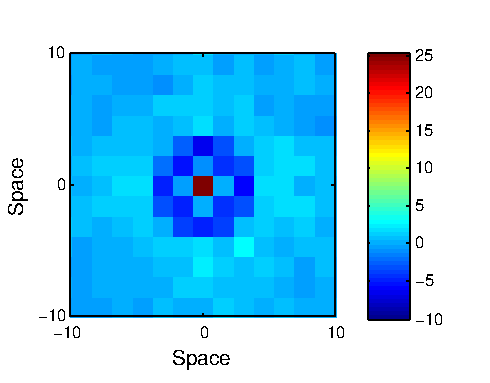
\includegraphics[scale=1]{KernelEstimateFullLinearizedPBC}}
		\subfigure[]{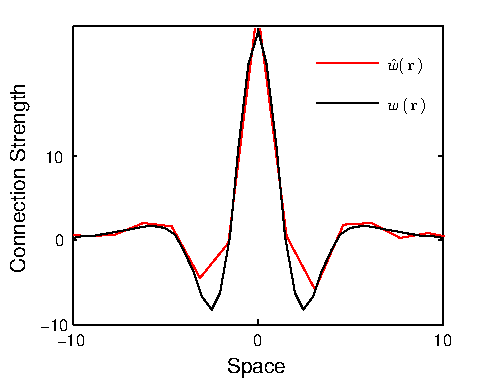
\includegraphics[scale=1]{KernelCrossSectionLinearizedPBC}}
	\caption{Linearized model to generate data. Linear model for estimation. Periodic boundary conditions.}
	\label{fig:label}
\end{figure}

\subsection{Nonlinear Neural Field Model}

\begin{figure}[htbp]
	\centering
		\subfigure[]{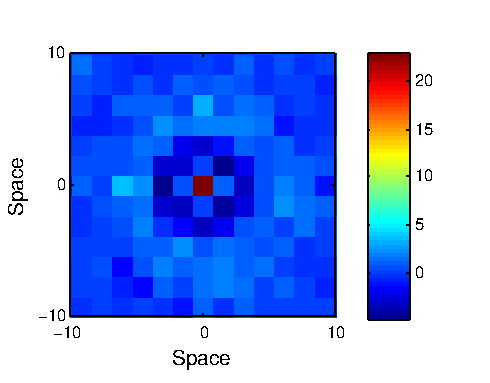
\includegraphics[scale=1]{KernelEstimateFullNonlinearPBC}}
		\subfigure[]{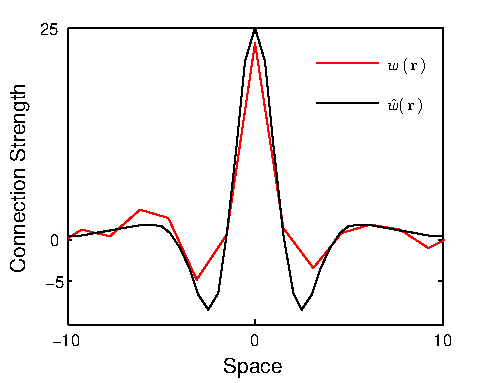
\includegraphics[scale=1]{KernelCrossSectionNonlinearPBC}}
	\caption{Nonlinear model to generate data. Linearized model for estimation. Periodic boundary conditions.}
	\label{fig:label}
\end{figure}
\newpage



\subsection{Linearized Neural Field Model}

\begin{figure}[htbp]
	\centering
		\subfigure[]{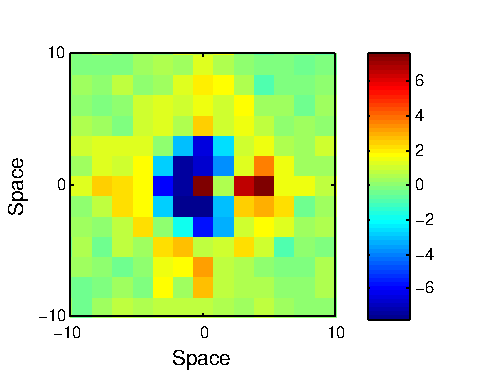
\includegraphics[scale=1]{KernelEstimateFullLinearizedPBCAniso}}
		\subfigure[]{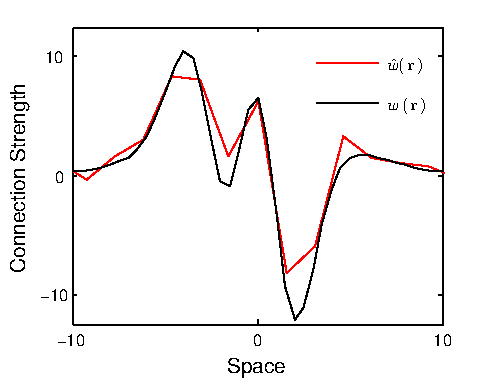
\includegraphics[scale=1]{KernelCrossSectionLinearizedPBCAniso}}
	\caption{Linearized model to generate data. Linear model for estimation. Periodic boundary conditions.}
	\label{fig:label}
\end{figure}

\subsection{Nonlinear Neural Field Model}

\begin{figure}[htbp]
	\centering
		\subfigure[]{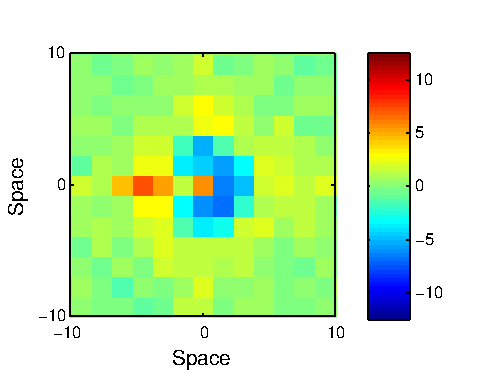
\includegraphics[scale=1]{KernelEstimateFullNonlinearPBCAniso}}
		\subfigure[]{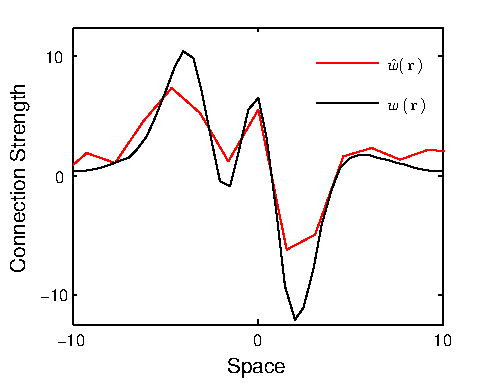
\includegraphics[scale=1]{KernelCrossSectionNonlinearPBCAniso}}
	\caption{Nonlinear model to generate data. Linearized model for estimation. Periodic boundary conditions.}
	\label{fig:label}
\end{figure}

\section{Discussion}

 


\section{Conclusion}
\subsection{The conclusion goes here.}




% conference papers do not normally have an appendix
\appendix
\section*{\parham{Convolution and Correlation}}
To show 
\begin{equation}
 \left(a \ast b \right)\left(\tau\right)  \star c\left(\tau\right)  = a\left(-\tau\right)\ast\left(b \star c\right)\left(\tau\right),
\end{equation}
we note that cross-correlation function is related to the convolution by \cite{Yarlagadda2009}
\begin{equation}
 \left(a \star b\right)\left(\tau\right)= a\left(-\tau \right)\ast b\left(\tau\right).
\end{equation}
Therefore, we can write
\begin{align}
 \left(a \ast b\right)\left(\tau\right) \star c\left(\tau\right)&= \left(a \ast b\right)\left(-\tau \right)\ast c\left(\tau\right) \nonumber \\
&=a\left(-\tau\right)\ast \left(b\left(-\tau\right) \ast c\left(\tau\right)\right)\nonumber \\
&=a\left(-\tau\right)\ast\left(b\star c\right)\left(\tau\right)
\end{align}



% use section* for acknowledgement
\section*{Acknowledgment}


The authors would like to thank...





\bibliographystyle{IEEEtran}
% argument is your BibTeX string definitions and bibliography database(s)
\bibliography{IEEEabrv,EMBC}


% that's all folks
\end{document}


